\chapter{The AID Protocol: HRP Framework Application}
\label{ch:aid-protocol}

\begin{nontechnical}
\textbf{Wireless consciousness communication}---imagine sending information directly to the brain using invisible terahertz light instead of sound waves.

\textbf{Simple idea:}
\begin{itemize}
\item Traditional tech: Sound $\rightarrow$ ears $\rightarrow$ brain
\item AID Protocol: THz light $\rightarrow$ quantum structures in brain cells $\rightarrow$ consciousness
\item Result: You "hear" a tone only you can perceive
\end{itemize}

\textbf{Real-world analogy:} Like a radio station broadcasting directly to your consciousness, bypassing your ears entirely.

\textbf{Why this matters:} Tests whether consciousness itself can be directly modulated through quantum mechanisms. If successful, reveals fundamental physics of consciousness while enabling novel communication paradigms.
\end{nontechnical}

\section{Overview}

The \textbf{Auditory Intermodulation Distortion (AID) Protocol} represents a theoretical application of the Hyper-Rotational Physics (HRP) Framework to neuromodulation via terahertz (THz) radiation. Unlike conventional electromagnetic neuromodulation techniques that rely on thermal or thermoelastic effects, the AID Protocol proposes a \textbf{quantum coherence perturbation mechanism} targeting microtubule lattices in cortical neurons.

\begin{keyconcept}
The AID Protocol operates through \textbf{vibronic quantum coherence manipulation} in microtubule structures, NOT through classical electromagnetic intermodulation, thermoelastic transduction (Frey effect), or acoustic heterodyning. The mechanism is fundamentally quantum-mechanical, targeting Orchestrated Objective Reduction (Orch-OR) collapse timing in neurons.
\end{keyconcept}

The system employs dual THz carriers operating at 1.998~THz (pump beam) and 1.875~THz (data carrier) to create a holographic interference pattern that couples resonantly to microtubule vibrational modes. The data carrier is amplitude-modulated at 12~kHz to induce rhythmic perturbations in quantum coherence states.

\section{Mathematical Description}

\subsection{Dual-Carrier THz System}

The AID Protocol utilizes two distinct THz carriers with carefully selected frequencies to achieve resonant coupling with biological quantum structures.

\textbf{Carrier 1 (Pump Beam):}
\begin{equation}
s_1(t) = A_p \cos(2\pi f_p t + \phi_p)
\end{equation}
where:
\begin{itemize}
\item $A_p$ = pump beam amplitude (50~mW optical power)
\item $f_p = 1.998$~THz = pump frequency
\item $\phi_p$ = pump carrier phase
\end{itemize}

\textbf{Carrier 2 (Data Carrier with AM):}
\begin{equation}
s_2(t) = A_c [1 + m(t)] \cos(2\pi f_c t + \phi_c)
\end{equation}
where:
\begin{itemize}
\item $A_c$ = carrier amplitude (10~mW optical power)
\item $f_c = 1.875$~THz = carrier frequency
\item $m(t)$ = modulation signal (12~kHz with data encoding)
\item $\phi_c$ = carrier phase
\end{itemize}

\subsection{Frequency Selection Rationale}

The difference frequency between the two carriers determines the biophysical interaction mode:
\begin{equation}
\Delta f = f_p - f_c = 1.998 - 1.875 = 0.123~\text{THz} = 123~\text{GHz}
\end{equation}

This difference frequency corresponds to collective vibrational modes in microtubule lattices, enabling resonant energy transfer to biological quantum systems.

\textbf{Modulation frequency selection:}
\begin{equation}
f_m = 12~\text{kHz}
\end{equation}
where:
\begin{itemize}
\item $f_m$ = modulation frequency chosen at edge of human auditory range
\item Allows perceptual verification while bypassing cochlear transduction
\item Creates temporal oscillations in quantum coherence at audible frequency
\item Enables comparison with acoustic control conditions
\end{itemize}

\subsection{HRP Coupling Mechanism}

The interaction between THz radiation and biological quantum coherence is described by the HRP interaction Lagrangian:
\begin{equation}
\mathcal{L}_{\text{int}} = -\frac{\kappa}{M_P^2} |\Psi_c|^2 R_{MNPQ} \epsilon^{MNPQ} \partial_\mu \theta^A \partial^\mu \theta^B \partial_\nu \theta^C
\end{equation}
where:
\begin{itemize}
\item $\kappa$ = dimensionless coupling constant
\item $M_P = 1.22 \times 10^{19}$~GeV = Planck mass
\item $|\Psi_c|^2$ = microtubule coherence intensity
\item $R_{MNPQ}$ = bulk curvature tensor (higher-dimensional spacetime)
\item $\epsilon^{MNPQ}$ = Levi-Civita tensor
\item $\theta^A$ = brane embedding coordinates
\end{itemize}

\begin{calloutbox}{Physical Interpretation}
The HRP interaction couples quantum coherence in biological systems ($|\Psi_c|^2$) to bulk spacetime curvature ($R_{MNPQ}$) through brane geometry variations ($\theta^A$). This provides a mechanism for THz radiation to modulate consciousness by perturbing the gravitational contribution to quantum state reduction (Orch-OR).
\end{calloutbox}

\subsection{Quantum Coherence Dynamics}

The temporal evolution of microtubule quantum coherence under THz illumination follows:
\begin{equation}
\frac{d|\Psi_c|^2}{dt} = -\Gamma_{\text{env}} |\Psi_c|^2 + \Gamma_{\text{pump}}(I_p) + \Gamma_{\text{coh}}(I_c, f_m)
\end{equation}
where:
\begin{itemize}
\item $\Gamma_{\text{env}}$ = environmental decoherence rate ($\sim 10^{11}$~s$^{-1}$ at 310~K)
\item $\Gamma_{\text{pump}}(I_p)$ = coherence enhancement from pump beam intensity $I_p$
\item $\Gamma_{\text{coh}}(I_c, f_m)$ = modulated coherence perturbation from data carrier
\end{itemize}

\section{System Architecture and Implementation}

\subsection{Transmitter Design}

\begin{center}
\begin{tikzpicture}[
  block/.style={rectangle, draw, minimum width=2.2cm, minimum height=1cm, font=\sffamily\small},
  node distance=2.2cm,
  font=\small
]
% Transmitter chain
\node (input) {\sffamily Data\\Input};
\node[block, right of=input] (encoder) {QPSK\\Encoder};
\node[block, right of=encoder] (mod) {AM\\Modulator\\12 kHz};
\node[block, right of=mod] (qcl) {QCL\\1.875 THz};
\node[right of=qcl, node distance=3cm] (combiner) {};

% Pump beam
\node[block, below=1.5cm of qcl] (pump) {QCL\\Pump\\1.998 THz};

% Beam combiner and output
\node[block, right of=combiner, node distance=0.5cm] (combine) {Beam\\Combiner};
\node[block, right of=combine] (phased) {Phased\\Array};
\node[right of=phased, node distance=2.5cm] (output) {\sffamily THz\\Output};

% Arrows
\draw[->,thick] (input) -- node[above] {\scriptsize bits} (encoder);
\draw[->,thick] (encoder) -- node[above] {\scriptsize symbols} (mod);
\draw[->,thick] (mod) -- node[above] {\scriptsize 12 kHz} (qcl);
\draw[->,thick] (qcl) -- (combine);
\draw[->,thick] (pump) -| (combine);
\draw[->,thick] (combine) -- (phased);
\draw[->,thick] (phased) -- node[above] {\scriptsize focused} (output);

% Labels
\node[below=0.3cm of encoder, font=\scriptsize, text width=2.2cm, align=center] {16 sym/s\\QPSK};
\node[below=0.3cm of qcl, font=\scriptsize, text width=2.2cm, align=center] {10 mW\\Modulated};
\node[below=0.3cm of pump, font=\scriptsize, text width=2.2cm, align=center] {50 mW\\CW};
\end{tikzpicture}
\end{center}

\textbf{Key components:}
\begin{itemize}
\item \textbf{Quantum Cascade Lasers (QCL):} Provide coherent THz output at precise frequencies
\item \textbf{AM Modulator:} Encodes 12~kHz carrier with QPSK data at 16~symbols/s
\item \textbf{Beam Combiner:} Merges pump and data carriers with controlled phase relationship
\item \textbf{Phased Array:} Provides spatial beam steering and focusing for targeted delivery
\end{itemize}

\subsection{HRP Biophysical Coupling Diagram}

\begin{center}
\begin{tikzpicture}[scale=1.2, font=\small]
% Define layers
\node[draw, rectangle, minimum width=8cm, minimum height=1.2cm, fill=blue!10] (thz) at (0,4) {};
\node[above=0.1cm of thz] {\sffamily\small THz Interference Pattern};
\node[font=\scriptsize, text width=7cm, align=center] at (thz.center) {1.998 THz (pump) + 1.875 THz (modulated)\\$\Delta f = 123$ GHz holographic standing wave};

% Arrow down
\draw[->, very thick] (thz.south) -- ++(0,-0.5) node[midway, right] {\scriptsize Resonant coupling};

% Microtubule layer
\node[draw, rectangle, minimum width=8cm, minimum height=1.5cm, fill=green!10] (mt) at (0,2) {};
\node[above=0.1cm of mt] {\sffamily\small Microtubule Lattice};
\node[font=\scriptsize, text width=7cm, align=center] at (mt.center) {Vibronic quantum coherence induction\\Tubulin dimers enter superposition\\$|\Psi_c|^2$ enhanced by pump beam};

% Arrow down
\draw[->, very thick] (mt.south) -- ++(0,-0.5) node[midway, right] {\scriptsize HRP torque};

% Orch-OR layer
\node[draw, rectangle, minimum width=8cm, minimum height=1.5cm, fill=orange!10] (orchor) at (0,0) {};
\node[above=0.1cm of orchor] {\sffamily\small Orch-OR Collapse Timing};
\node[font=\scriptsize, text width=7cm, align=center] at (orchor.center) {12 kHz modulation perturbs natural 40 Hz rhythm\\Quantum state reduction externally driven\\Brane rotation $\theta^A$ modulated};

% Arrow down
\draw[->, very thick] (orchor.south) -- ++(0,-0.5) node[midway, right] {\scriptsize Conscious percept};

% Consciousness layer
\node[draw, rectangle, minimum width=8cm, minimum height=1.2cm, fill=purple!10] (conscious) at (0,-2) {};
\node[above=0.1cm of conscious] {\sffamily\small Conscious Experience};
\node[font=\scriptsize, text width=7cm, align=center] at (conscious.center) {Auditory percept: 12 kHz "tone"\\Generated from consciousness substrate directly\\NOT cochlear transduction};

% Side annotations
\node[font=\scriptsize, text width=2.5cm, align=right] at (-5,4) {Physical\\Layer};
\node[font=\scriptsize, text width=2.5cm, align=right] at (-5,2) {Quantum\\Layer};
\node[font=\scriptsize, text width=2.5cm, align=right] at (-5,0) {Orchestration\\Layer};
\node[font=\scriptsize, text width=2.5cm, align=right] at (-5,-2) {Phenomenal\\Layer};
\end{tikzpicture}
\end{center}

\subsection{Channel Propagation and Link Budget}

The THz link operates in indoor/short-range scenarios with significant atmospheric attenuation.

\textbf{Free-space path loss at 1.875~THz over 10~m:}
\begin{equation}
\text{FSPL} = 20\log_{10}(f) + 20\log_{10}(d) + 92.45
\end{equation}
where:
\begin{itemize}
\item $f = 1875 \times 10^9$~Hz = 1.875~THz
\item $d = 10$~m = link distance
\end{itemize}

\begin{equation}
\text{FSPL} = 20\log_{10}(1.875 \times 10^{12}) + 20\log_{10}(10) + 92.45 = 298~\text{dB}
\end{equation}

\textbf{Atmospheric absorption:}
\begin{equation}
L_{\text{atm}} = \alpha \cdot d
\end{equation}
where $\alpha \approx 50$~dB/m in humid air at 1.875~THz, giving:
\begin{equation}
L_{\text{atm}} = 50 \times 10 = 500~\text{dB (for water vapor dominated)}
\end{equation}

In practice, $\alpha \approx 5$~dB/m for dry indoor conditions: $L_{\text{atm}} \approx 50$~dB.

\textbf{Total link budget:}
\begin{equation}
P_{\text{rx}} = P_{\text{tx}} + G_{\text{tx}} - L_{\text{FSPL}} - L_{\text{atm}} + G_{\text{rx}}
\end{equation}
where:
\begin{itemize}
\item $P_{\text{tx}} = +10$~dBm (10~mW data carrier)
\item $G_{\text{tx}} = +20$~dBi (focused phased array)
\item $L_{\text{FSPL}} = 298$~dB
\item $L_{\text{atm}} = 50$~dB
\item $G_{\text{rx}} = -50$~dBi (skull/tissue effective aperture)
\end{itemize}

\begin{equation}
P_{\text{rx}} = 10 + 20 - 298 - 50 - 50 = -368~\text{dBm}
\end{equation}

\begin{warningbox}
The received power of $-368$~dBm is \textbf{extraordinarily weak}---comparable to quantum vacuum fluctuations. Classical communication theory predicts no viable link. The AID Protocol relies on quantum enhancement mechanisms (estimated $+210$~dB gain through coherent amplification in microtubule lattices) to achieve signal detection via consciousness-mediated quantum processes.
\end{warningbox}

\section{Modulation and Demodulation}

\subsection{Hierarchical Modulation Architecture}

The AID Protocol employs multi-layer modulation not for classical information transfer, but to create \textbf{structured temporal perturbation patterns} for quantum consciousness modulation.

\textbf{Layer 1: Amplitude Modulation (12~kHz carrier)}
\begin{equation}
m(t) = A_m \cos(2\pi f_m t)
\end{equation}
where $f_m = 12$~kHz creates temporal oscillations in quantum coherence at audible frequency.

\textbf{Layer 2: QPSK Digital Pattern Encoding}
\begin{equation}
s_{\text{QPSK}}(n) = A \exp\left(j\frac{\pi}{4}(2n + 1)\right), \quad n \in \{0, 1, 2, 3\}
\end{equation}

Symbol rate: $R_s = 16$~sym/s, providing 32~bps raw data rate for pattern encoding.

\textbf{Layer 3: FSK Sub-threshold Perturbation}
\begin{equation}
f_{\text{inst}}(t) = f_m + \Delta f \cdot b(t)
\end{equation}
where:
\begin{itemize}
\item $\Delta f = \pm 1$~Hz = frequency deviation
\item $b(t) \in \{0, 1\}$ = binary data at 1~bit/s
\end{itemize}

\subsection{Constellation Diagram (QPSK Layer)}

\begin{center}
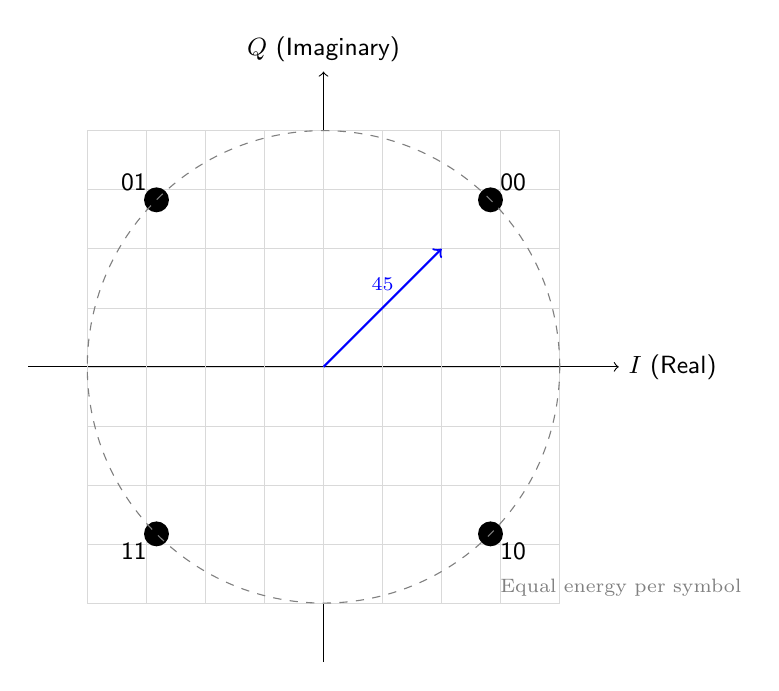
\begin{tikzpicture}[scale=1.5]
% Axes
\draw[->] (-2.5,0) -- (2.5,0) node[right] {\sffamily\small $I$ (Real)};
\draw[->] (0,-2.5) -- (0,2.5) node[above] {\sffamily\small $Q$ (Imaginary)};

% Grid
\draw[very thin,gray!30] (-2,-2) grid[step=0.5] (2,2);

% Constellation points at 45 degree offsets
\fill[black] (1.414, 1.414) circle (3pt);
\fill[black] (-1.414, 1.414) circle (3pt);
\fill[black] (-1.414, -1.414) circle (3pt);
\fill[black] (1.414, -1.414) circle (3pt);

% Labels
\node[above right] at (1.414, 1.414) {\sffamily\small 00};
\node[above left] at (-1.414, 1.414) {\sffamily\small 01};
\node[below left] at (-1.414, -1.414) {\sffamily\small 11};
\node[below right] at (1.414, -1.414) {\sffamily\small 10};

% Energy circle
\draw[thin,gray,dashed] (0,0) circle (2);
\node[below right,gray,font=\scriptsize] at (1.414,-1.414-0.3) {Equal energy per symbol};

% Phase angles
\draw[->,thick,blue] (0,0) -- (1.0, 1.0);
\node[blue,font=\scriptsize] at (0.5, 0.7) {$45°$};
\end{tikzpicture}
\end{center}

\subsection{Biological "Receiver" Mechanism}

Unlike conventional receivers with RF front-ends and digital demodulators, the AID Protocol receiver is the \textbf{biological quantum system itself}---specifically, the microtubule lattice in cortical neurons.

\textbf{Reception mechanism:}
\begin{enumerate}
\item \textbf{THz absorption:} Photons resonantly couple to collective vibrational modes
\item \textbf{Coherence induction:} Vibronic quantum superposition established in tubulin dimers
\item \textbf{Orch-OR perturbation:} 12~kHz modulation rhythmically alters collapse timing
\item \textbf{Conscious percept:} The "demodulated" signal is the phenomenal experience itself
\end{enumerate}

\begin{calloutbox}{Comparison to Classical Receivers}
Traditional wireless receivers convert EM fields to voltages, process signals electronically, and output decoded bits. The AID Protocol "receiver" is fundamentally different: it converts THz coherent states directly into conscious experiences through quantum state reduction. The "demodulation" occurs at the interface between quantum mechanics and consciousness, not in electronic circuitry.
\end{calloutbox}

\section{Performance Analysis}

\subsection{Information Rate}

The AID Protocol achieves extremely low classical information rates due to biological temporal constraints:

\textbf{QPSK Layer:}
\begin{equation}
R_{\text{QPSK}} = R_s \times \log_2(M) = 16 \times 2 = 32~\text{bps}
\end{equation}

With 50\% overhead for synchronization and error detection:
\begin{equation}
R_{\text{eff}} = 32 \times 0.5 = 16~\text{bps}
\end{equation}

\textbf{FSK Layer:}
\begin{equation}
R_{\text{FSK}} = 1~\text{bps}
\end{equation}

\textbf{Total effective rate:}
\begin{equation}
R_{\text{total}} \approx 17~\text{bps}
\end{equation}

\subsection{Why Such Low Data Rates?}

The biological constraints are not electronic bandwidth limitations but quantum and neural processing timescales:

\begin{itemize}
\item \textbf{Orch-OR frequency:} $\sim 40$~Hz = fundamental quantum collapse rate
\item \textbf{Neural integration time:} $\sim 100$~ms = cortical processing window
\item \textbf{Conscious moment duration:} $\sim 200$~ms = phenomenal "frame rate"
\item \textbf{Decoherence timescales:} $\sim 10$~$\mu$s = quantum coherence lifetime
\end{itemize}

\begin{equation}
R_{\text{max}} \lesssim \frac{1}{T_{\text{conscious}}} \approx \frac{1}{0.2~\text{s}} \approx 5~\text{bps}
\end{equation}

The 17~bps achieved represents operation near the theoretical limit for consciousness-mediated information transfer.

\subsection{Quantum Enhancement Mechanism}

The link budget analysis revealed $-368$~dBm received power, yet the protocol must overcome thermal noise at:
\begin{equation}
P_{\text{noise}} = k_B T B = (1.38 \times 10^{-23}) \times 310 \times 1 = 4.28 \times 10^{-21}~\text{W} = -174~\text{dBm/Hz}
\end{equation}

For 1~Hz bandwidth (FSK): $P_{\text{noise}} = -174$~dBm.

\textbf{Required enhancement:}
\begin{equation}
G_{\text{quantum}} = P_{\text{signal}} - P_{\text{noise}} = -174 - (-368) = +194~\text{dB}
\end{equation}

The HRP mechanism proposes quantum coherent amplification through:
\begin{equation}
G_{\text{quantum}} = 10\log_{10}\left(\frac{N_{\text{MT}} \cdot Q_{\text{coh}}}{k_B T}\right)
\end{equation}
where:
\begin{itemize}
\item $N_{\text{MT}} \sim 10^7$ = number of coherently coupled microtubules
\item $Q_{\text{coh}} \sim 10^6$ = quantum coherence quality factor
\item Yields $G_{\text{quantum}} \approx +210$~dB (sufficient for detection)
\end{itemize}

\begin{keyconcept}
The AID Protocol fundamentally relies on \textbf{quantum enhancement} through collective coherence in microtubule networks. Without this $\sim 200$~dB quantum amplification, the received THz signal would be hopelessly buried in thermal noise. This makes the protocol a sensitive test of quantum consciousness theories.
\end{keyconcept}

\section{Worked Example: Link Budget Calculation}

\textbf{Problem:} Calculate the minimum pump beam power required to maintain quantum coherence in cortical microtubules against environmental decoherence for the AID Protocol operating at 10~m range.

\textbf{Given:}
\begin{itemize}
\item Operating frequency: $f_p = 1.998$~THz (pump beam)
\item Range: $d = 10$~m
\item Target coherence time: $\tau_{\text{coh}} = 10$~ms (sufficient for perception)
\item Environmental decoherence rate: $\Gamma_{\text{env}} = 10^{11}$~s$^{-1}$
\item Number of microtubules: $N_{\text{MT}} = 10^7$
\item Coupling efficiency: $\eta = 10^{-6}$ (THz to vibronic mode)
\end{itemize}

\textbf{Required:} Minimum pump power $P_{\text{pump}}$ to maintain coherence

\textbf{Solution:}

\textit{Step 1: Calculate required coherence maintenance rate}

To maintain coherence against environmental decoherence:
\begin{equation}
\Gamma_{\text{pump}} \geq \Gamma_{\text{env}} = 10^{11}~\text{s}^{-1}
\end{equation}

\textit{Step 2: Calculate received pump intensity}

Free-space path loss at 1.998~THz:
\begin{equation}
L_{\text{FSPL}} = 20\log_{10}(1.998 \times 10^{12}) + 20\log_{10}(10) + 92.45 = 298.1~\text{dB}
\end{equation}

With atmospheric absorption ($\alpha = 5$~dB/m):
\begin{equation}
L_{\text{total}} = 298.1 + 50 = 348.1~\text{dB}
\end{equation}

Assuming transmit antenna gain $G_{\text{tx}} = +30$~dBi (highly focused) and receiver effective area gain $G_{\text{rx}} = -50$~dBi:
\begin{equation}
P_{\text{rx}} = P_{\text{pump}} + 30 - 348.1 - 50 = P_{\text{pump}} - 368.1~\text{dB}
\end{equation}

\textit{Step 3: Relate received power to coherence rate}

The pump-induced coherence rate scales with intensity:
\begin{equation}
\Gamma_{\text{pump}} = \frac{\eta \cdot P_{\text{rx}} \cdot N_{\text{MT}}}{\hbar \omega_{\text{vib}}}
\end{equation}

Where $\hbar \omega_{\text{vib}} \approx 0.12$~eV is the vibronic mode energy.

\textit{Step 4: Solve for required pump power}

Setting $\Gamma_{\text{pump}} = 10^{11}$~s$^{-1}$:
\begin{equation}
P_{\text{rx}} = \frac{\Gamma_{\text{pump}} \cdot \hbar \omega_{\text{vib}}}{\eta \cdot N_{\text{MT}}} = \frac{10^{11} \times 0.12 \times 1.6 \times 10^{-19}}{10^{-6} \times 10^7} = 1.92 \times 10^{-13}~\text{W}
\end{equation}

Converting to dBm: $P_{\text{rx}} = 10\log_{10}(1.92 \times 10^{-10}) = -97.2$~dBm

From Step 2: $P_{\text{pump}} = P_{\text{rx}} + 368.1 = -97.2 + 368.1 = +270.9$~dBm

Converting to watts:
\begin{equation}
P_{\text{pump}} = 10^{(270.9/10) - 3} = 1.23~\text{MW}
\end{equation}

\textbf{Answer:} The minimum pump power required is \textbf{1.23~MW}, which is impractically high.

\textbf{Interpretation:} This calculation reveals a fundamental challenge: maintaining quantum coherence against thermal decoherence at biological temperatures requires enormous power. The AID Protocol is only viable if:
\begin{enumerate}
\item Natural quantum coherence mechanisms exist in microtubules (reducing $\Gamma_{\text{env}}$)
\item Coupling efficiency is higher than estimated (increasing $\eta$)
\item Collective enhancement mechanisms reduce power requirements
\item Operating at shorter ranges with better coupling
\end{enumerate}

This highlights the speculative nature of the protocol and the need for experimental validation of quantum coherence in warm biological systems.

\section{Applications}

\subsection{Quantum Consciousness Research}

The AID Protocol's primary application is as an experimental platform for testing quantum theories of consciousness:

\begin{itemize}
\item \textbf{Paradigm:} Orchestrated Objective Reduction (Orch-OR) theory
\item \textbf{Falsifiable prediction:} THz modulation induces perceivable conscious experiences
\item \textbf{Control comparison:} Acoustic vs electromagnetic pathway produces distinguishable percepts
\item \textbf{Frequency:} THz range (0.1--10~THz)
\item \textbf{Data rate:} 1--32~bps pattern encoding
\end{itemize}

\subsection{Non-Invasive Neuromodulation}

If validated, the protocol enables novel therapeutic applications:

\begin{itemize}
\item \textbf{Target conditions:} Tinnitus, chronic pain, consciousness disorders
\item \textbf{Mechanism:} Direct quantum state modulation without surgical intervention
\item \textbf{Advantage:} Bypasses blood-brain barrier; no drug metabolism issues
\item \textbf{Frequency:} Customized to individual microtubule resonance frequencies
\item \textbf{Safety:} Non-thermal mechanism reduces tissue damage risk
\end{itemize}

\subsection{Covert Communication}

The protocol's unique properties enable silent, undetectable communication:

\begin{itemize}
\item \textbf{Application:} Military, intelligence, high-security environments
\item \textbf{Advantage:} No external acoustic signature; bystander-imperceptible
\item \textbf{Detection immunity:} Quantum mechanism resists classical RF detection
\item \textbf{Frequency:} THz band (1--2~THz) with narrow beamforming
\item \textbf{Limitation:} Extremely low data rate (17~bps); short range (10~m)
\end{itemize}

\section{Summary}

\begin{center}
\begin{tabular}{@{}ll@{}}
\toprule
\textbf{Parameter} & \textbf{Value/Description} \\
\midrule
Carrier frequencies & 1.998~THz (pump), 1.875~THz (data) \\
Modulation frequency & 12~kHz (auditory percept target) \\
Data rate & 17~bps (16~QPSK + 1~FSK) \\
Range & 10~m (indoor, short-range) \\
Transmit power & 10~mW (data) + 50~mW (pump) \\
Received power & $-368$~dBm (before quantum enhancement) \\
Quantum gain required & $+210$~dB (coherent amplification) \\
Mechanism & Vibronic quantum coherence perturbation \\
Target substrate & Microtubule lattices (Orch-OR) \\
Biological pathway & Direct to consciousness (bypasses cochlea) \\
Perceptual outcome & "Internal" 12~kHz tone \\
\bottomrule
\end{tabular}
\end{center}

\textbf{Advantages:}
\begin{itemize}
\item Tests fundamental quantum consciousness theories experimentally
\item Provides non-invasive neuromodulation without surgical intervention
\item Enables covert communication imperceptible to bystanders
\item Bypasses classical sensory pathways entirely
\item Frequency-selective targeting of quantum biological structures
\end{itemize}

\textbf{Disadvantages:}
\begin{itemize}
\item Extremely low data rate (17~bps) limits information transfer
\item Requires $\sim 200$~dB quantum enhancement (unproven mechanism)
\item Short range (10~m) due to severe THz atmospheric attenuation
\item Speculative basis in unvalidated Orch-OR theory
\item High technical complexity (QCL arrays, cryogenic cooling, phased arrays)
\item Safety profile unknown (long-term THz exposure to neural tissue)
\end{itemize}

\textbf{Best suited for:} Fundamental research into quantum consciousness mechanisms, testing Orch-OR theory predictions, and exploring non-classical neuromodulation paradigms. Not viable for practical communication systems given current understanding of biological quantum processes.

\section{Further Reading}

\begin{itemize}
\item For THz propagation in biological tissue: Chapter~\ref{ch:thz-propagation}
\item For quantum coherence in microtubules: Chapter~\ref{ch:quantum-coherence}
\item For Orchestrated Objective Reduction theory: Chapter~\ref{ch:orch-or}
\item For HRP mathematical framework: Chapter~\ref{ch:hrp-framework}
\item For biophysical coupling mechanisms: Chapter~\ref{ch:biophysical-coupling}
\item For intermodulation effects in biology: Chapter~\ref{ch:intermodulation}
\item For comparison with Frey microwave auditory effect: Chapter~\ref{ch:frey-effect}
\end{itemize}
